\documentclass[10pt,aspectratio=169,serif,fleqn]{beamer}

\usepackage[fontset=none, scheme=plain]{ctex}
\IfFontExistsTF{Songti SC}{%
	\setCJKmainfont{Songti SC}[AutoFakeSlant=0.2]%
	\setCJKsansfont{Songti SC}[AutoFakeSlant=0.2]%
}{%
	\setCJKmainfont{FandolSong-Regular}[Extension=.otf,BoldFont=FandolSong-Bold,AutoFakeSlant=0.2]%
	\setCJKsansfont{FandolSong-Regular}[Extension=.otf,BoldFont=FandolSong-Bold]%
}
\usepackage{amsmath,amssymb,graphicx,tikz,booktabs,multicol,calligra}
\usepackage{pgfplots}
\pgfplotsset{compat=1.18}
\usepackage{tcolorbox}
\tcbuselibrary{skins}
\usepackage{XyygU}
\usepackage{caption}
\captionsetup[figure]{name=图,labelsep=period}

\usetikzlibrary{arrows.meta,positioning,calc,intersections}

\setlength{\abovedisplayskip}{0pt plus 2pt minus 2pt}
\setlength{\belowdisplayskip}{0pt plus 2pt minus 2pt}

\title[复习参考题3]{复习参考题3 \quad 函数的概念与性质}
\subtitle{复习巩固 \& 综合运用 \& 拓广探索}
\author{}
\institute{}
\date{2026-10-31}

\begin{document}

\begin{frame}
  \titlepage
\end{frame}

% ========== 第1题 ==========
\begin{frame}[t]{第1题：求函数定义域}
\textbf{1.} 求下列函数的定义域：

\vspace{0.5em}
(1) $y=\sqrt{x-2}\sqrt{x+5}$；\hfil (2) $y=\dfrac{\sqrt{x-4}}{|x|-5}$。
\end{frame}

\begin{frame}[t]{第1题 解答}
\begin{tcolorbox}[colback=orange!10,colframe=orange,title=\textbf{解}]
(1) 需 $\begin{cases}x-2\ge0\\ x+5\ge0\end{cases}$，即 $x\ge2$。

\vspace{0.3em}
定义域：$\alert{[2,+\infty)}$。

\vspace{0.8em}
(2) 需 $\begin{cases}x-4\ge0\\ |x|-5\ne0\end{cases}$，即 $x\ge4$ 且 $x\ne5$。

\vspace{0.3em}
定义域：$\alert{[4,5)\cup(5,+\infty)}$。
\end{tcolorbox}
\end{frame}

% ========== 第2题 ==========
\begin{frame}[t]{第2题：求函数值}
\textbf{2.} 已知函数 $f(x)=\dfrac{1-x}{1+x}$，求：

\vspace{0.5em}
(1) $f(a)+1\ (a\ne-1)$；\hfil (2) $f(a+1)\ (a\ne-2)$。
\end{frame}

\begin{frame}[t]{第2题 解答}
\begin{tcolorbox}[colback=orange!10,colframe=orange,title=\textbf{解}]
(1)
\[
f(a)+1=\frac{1-a}{1+a}+1=\frac{1-a+1+a}{1+a}=\alert{\frac{2}{1+a}}.
\]

\vspace{0.8em}
(2)
\[
f(a+1)=\frac{1-(a+1)}{1+(a+1)}=\frac{-a}{a+2}=\alert{-\frac{a}{a+2}}.
\]
\end{tcolorbox}
\end{frame}

% ========== 第3题 ==========
\begin{frame}[t]{第3题：证明函数恒等式}
\textbf{3.} 设 $f(x)=\dfrac{1+x^2}{1-x^2}$，求证：

\vspace{0.5em}
(1) $f(-x)=f(x)$；\hfil (2) $f\!\left(\dfrac1x\right)=-f(x)\ (x\ne0)$。
\end{frame}

\begin{frame}[t]{第3题 解答}
\begin{tcolorbox}[colback=orange!10,colframe=orange,title=\textbf{证明}]
(1)
\[
f(-x)=\frac{1+(-x)^2}{1-(-x)^2}=\frac{1+x^2}{1-x^2}=f(x).
\]

\vspace{0.8em}
(2)
\[
f\!\left(\frac1x\right)=\frac{1+\frac1{x^2}}{1-\frac1{x^2}}=\frac{x^2+1}{x^2-1}=-\frac{1+x^2}{1-x^2}=-f(x).
\]
\end{tcolorbox}
\end{frame}

% ========== 第4题 ==========
\begin{frame}[t]{第4题：二次函数在区间上单调}
\textbf{4.} 已知函数 $f(x)=4x^2-kx-8$ 在 $[5,20]$ 上具有单调性，求实数 $k$ 的取值范围。
\end{frame}

\begin{frame}[t]{第4题 解答}
\begin{tcolorbox}[colback=orange!10,colframe=orange,title=\textbf{解}]
$f(x)=4x^2-kx-8$ 的对称轴为
\[
x=\frac{k}{8}.
\]
抛物线开口向上。要使 $f(x)$ 在 $[5,20]$ 上单调，区间 $[5,20]$ 必须完全在对称轴的一侧。

\vspace{0.5em}
即 $\dfrac{k}{8}\le5$ 或 $\dfrac{k}{8}\ge20$。

\vspace{0.3em}
解得 $k\le40$ 或 $k\ge160$。

\vspace{0.5em}
故 $k$ 的取值范围为 $\alert{(-\infty,40]\cup[160,+\infty)}$。
\end{tcolorbox}
\end{frame}

% ========== 第5题 ==========
\begin{frame}[t]{第5题：幂函数过定点}
\textbf{5.} 已知幂函数 $y=f(x)$ 的图象过点 $\left(2,\dfrac{\sqrt{2}}{2}\right)$，试求出此函数的解析式，并画出图象，判断奇偶性、单调性。
\end{frame}

\begin{frame}[t]{第5题 解答}
	
\vspace{-2em}
\begin{tcolorbox}[colback=orange!10,colframe=orange,title=\textbf{解}]
设 $f(x)=x^{\alpha}$，代入 $\left(2,\dfrac{\sqrt{2}}{2}\right)$：
\[
2^{\alpha}=\frac{\sqrt2}{2}=2^{-\frac12},\quad \alpha=-\frac12.
\]
故
\[
f(x)=x^{-\frac12}=\frac{1}{\sqrt{x}}.
\]

\vspace{0.3em}
\textbf{定义域：} $(0,+\infty)$，不关于原点对称，故 \alert{既不是奇函数也不是偶函数}。

\vspace{0.3em}
在 $(0,+\infty)$ 上，$x$ 增大时 $\dfrac{1}{\sqrt{x}}$ 减小，故 $f(x)$ 在 $(0,+\infty)$ 上 \alert{单调递减}。
\end{tcolorbox}
\end{frame}

\begin{frame}[t]{第5题 图象}
\begin{center}
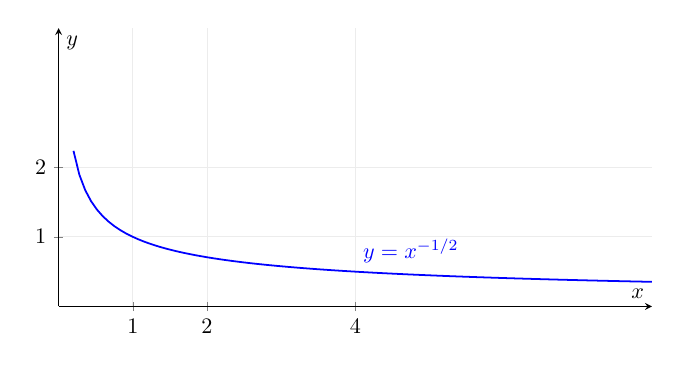
\begin{tikzpicture}[scale=0.8]
\begin{axis}[
    width=11cm, height=6cm,
    axis lines=middle,
    xlabel=$x$, ylabel=$y$,
    xmin=0, xmax=8, ymin=0, ymax=4,
    xtick={1,2,4},
    ytick={1,2},
    grid=major, grid style={gray!15},
]
\addplot[thick,blue,domain=0.2:8,samples=100] {1/sqrt(x)};
\node[blue,right] at (axis cs:4,0.8) {$y=x^{-1/2}$};
\end{axis}
\end{tikzpicture}
\end{center}
\end{frame}

% ========== 第6题 ==========
\begin{frame}[t]{第6题：电子仪器利润}
\textbf{6.} 某公司生产某种电子仪器的固定成本为 $20000$ 元，每生产一台仪器需增加投入 $100$ 元，已知总收入 $R$（单位：元）关于月产量 $x$（单位：台）满足函数：
\[
R=\begin{cases}
400x-\dfrac12x^2, & 0\le x\le400,\\
80000, & x\ge400.
\end{cases}
\]
(1) 将利润 $P$（单位：元）表示为月产量 $x$ 的函数；

(2) 当月产量为何值时，公司所获利润最大？最大利润为多少元？（总收入 $=$ 总成本 $+$ 利润）
\end{frame}

\begin{frame}[t]{第6题 解答}\vspace{-2em}
\begin{tcolorbox}[colback=orange!10,colframe=orange,title=\textbf{解}]
总成本 $C=20000+100x$，利润 $P=R-C$。

\vspace{0.3em}
(1) 当 $0\le x\le400$ 时：
\[
P=400x-\frac12x^2-(20000+100x)=-\frac12x^2+300x-20000.
\]
当 $x\ge400$ 时：
\[
P=80000-(20000+100x)=60000-100x.
\]

\vspace{0.5em}
(2) 当 $0\le x\le400$ 时，$P=-\frac12(x-300)^2+25000$，$x=300$ 时 $P_{\max}=25000$ 元；

当 $x\ge400$ 时，$P=60000-100x$ 递减，$P\le20000$ 元。

\vspace{0.3em}
故月产量为 \alert{300 台}时利润最大，最大利润为 \alert{25000 元}。
\end{tcolorbox}
\end{frame}

% ========== 第7题 ==========
\begin{frame}[t]{第7题：分段函数求值}
\textbf{7.} 已知函数
\[
f(x)=\begin{cases}
x(x+4), & x\ge0,\\
x(x-4), & x <0,
\end{cases}
\]
求 $f(1)$，$f(-3)$，$f(a+1)$ 的值。
\end{frame}

\begin{frame}[t]{}\vspace{-1em}
\begin{tcolorbox}[colback=orange!10,colframe=orange,title=\textbf{解}]
\textbf{$f(1)$：} $1\ge0$，$f(1)=1\times(1+4)=5$。

\vspace{0.5em}
\textbf{$f(-3)$：} $-3< 0$，$f(-3)=(-3)\times(-3-4)=21$。

\vspace{0.5em}
\textbf{$f(a+1)$：} 需分情况：
\begin{itemize}
  \item 当 $a+1\ge0$，即 $a\ge-1$ 时，
  \[
  f(a+1)=(a+1)(a+5)=a^2+6a+5;
  \]
  \item 当 $a+1< 0$，即 $a\le-1$ 时，
  \[
  f(a+1)=(a+1)(a+1-4)=(a+1)(a-3)=a^2-2a-3.
  \]
  因此$f(a+1) =
  \begin{cases}
  	a^2 +6a+5,&a \geqslant -1\\
  		a^2 -2a -3,&a<-1\\ 	
  \end{cases}$
\end{itemize}
\end{tcolorbox}
\end{frame}

% ========== 第8题 ==========
\begin{frame}[t]{第8题：中点函数值}
\textbf{8.} 证明：

(1) 若 $f(x)=ax+b$，则 $f\!\left(\dfrac{x_1+x_2}{2}\right)=\dfrac{f(x_1)+f(x_2)}{2}$；

(2) 若 $g(x)=x^2+ax+b$，则 $g\!\left(\dfrac{x_1+x_2}{2}\right)\le\dfrac{g(x_1)+g(x_2)}{2}$。
\end{frame}

\begin{frame}[t]{第8题 解答}\vspace{-2em}
\begin{tcolorbox}[colback=orange!10,colframe=orange,title=\textbf{证明}]
\[(1)
f\!\left(\frac{x_1+x_2}{2}\right)=a\frac{x_1+x_2}{2}+b,
\]
\[
\frac{f(x_1)+f(x_2)}{2}=\frac{(ax_1+b)+(ax_2+b)}{2}=a\frac{x_1+x_2}{2}+b,
\]
两边相等。

\end{tcolorbox}
\end{frame}

\begin{frame}
	
	\begin{tcolorbox}[colback=orange!10,colframe=orange,title=\textbf{证明}]
	(2)$g(\dfrac{x_1+x_2}{2})
	=\dfrac{(x_1+x_2)^2}{4}+a\cdot\dfrac{x_1+x_2}{2}+b
	=\dfrac{x_1^2+2x_1x_2+x_2^2}{4}+\dfrac{a(x_1+x_2)}{2}+b.$ \\[2pt]
		
	$\dfrac{g(x_1)+g(x_2)}{2}
	=\dfrac{(x_1^2+ax_1+b)+(x_2^2+ax_2+b)}{2}
	=\dfrac{x_1^2+x_2^2}{2}+\dfrac{a(x_1+x_2)}{2}+b.$ \\[2pt]
	
	$\dfrac{g(x_1)+g(x_2)}{2}-g\!\left(\dfrac{x_1+x_2}{2}\right)
	=\dfrac{x_1^2+x_2^2}{2}-\dfrac{x_1^2+2x_1x_2+x_2^2}{4}.$\\[2pt]
	
	$	=\dfrac{2x_1^2+2x_2^2-(x_1^2+2x_1x_2+x_2^2)}{4}
	=\dfrac{x_1^2-2x_1x_2+x_2^2}{4}
	=\dfrac{(x_1-x_2)^2}{4}.$\\[2pt]
	
	由于 \((x_1-x_2)^2\ge 0\)，所以
	$\dfrac{g(x_1)+g(x_2)}{2}-g\!\left(\dfrac{x_1+x_2}{2}\right)\ge 0,$
	
	故$	g\!\left(\dfrac{x_1+x_2}{2}\right)\le\dfrac{g(x_1)+g(x_2)}{2}.$
	
	
	等号成立当且仅当 \(x_1=x_2\)。
	\end{tcolorbox}
\end{frame}

% ========== 第9题 ==========
\begin{frame}[t]{第9题：奇偶函数对称区间单调性}
\textbf{9.} (1) 已知奇函数 $f(x)$ 在 $[a,b]$ 上单调递减，那么它在 $[-b,-a]$ 上单调递增还是单调递减？

\vspace{0.5em}
(2) 已知偶函数 $g(x)$ 在 $[a,b]$ 上单调递减，那么它在 $[-b,-a]$ 上单调递增还是单调递减？
\end{frame}

\begin{frame}[t]{第9题 解答}
\begin{tcolorbox}[colback=orange!10,colframe=orange,title=\textbf{解}]
(1) 任取 $-b\le x_1\le x_2\le-a$，则 $a\le -x_2\le -x_1\le b$。

\vspace{0.3em}
因 $f$ 在 $[a,b]$ 递减，$f(-x_2)\ge f(-x_1)$。又 $f$ 为奇函数，
\[
-f(x_2)\ge-f(x_1)\Rightarrow f(x_2)\le f(x_1),
\]
即 $f(x_1)\ge f(x_2)$，故 $f$ 在 $[-b,-a]$ 上 \alert{单调递减}（与 $[a,b]$ 上单调性相同）。

\vspace{0.8em}
(2) 任取 $-b\le x_1\le x_2\le-a$，则 $a\le -x_2\le -x_1\le b$。

\vspace{0.3em}
$g$ 在 $[a,b]$ 递减，$g(-x_2)\ge g(-x_1)$。又 $g$ 为偶函数，$g(x_2)\ge g(x_1)$，即 $g(x_1)\le g(x_2)$，故 $g$ 在 $[-b,-a]$ 上 \alert{单调递增}（与 $[a,b]$ 上单调性相反）。
\end{tcolorbox}
\end{frame}

% ========== 第10题 ==========
\begin{frame}[t]{第10题：电价调整}
\textbf{10.} 某地区上年度电价为 $0.8$ 元/(kW$\cdot$h)，年用电量为 $a$ kW$\cdot$h，本年度计划将电价下降到 $0.55$ 元/(kW$\cdot$h) 至 $0.75$ 元/(kW$\cdot$h) 之间，而用户期望电价为 $0.4$ 元/(kW$\cdot$h)。经测算，下调电价后新增用电量和实际电价与用户的期望电价的差成反比（比例系数为 $k$）。该地区的电力成本价为 $0.3$ 元/(kW$\cdot$h)。

(1) 写出本年度电价下调后电力部门的收益 $y$ 关于实际电价 $x$ 的函数解析式；（收益 $=$ 实际电量 $\times$（实际电价 $-$ 成本价））

(2) 设 $k=0.2a$，当电价最低定为多少时，仍可保证电力部门的收益比上年至少增长 $20\%$？
\end{frame}

\begin{frame}[t]{}\vspace{-1em}
\begin{tcolorbox}[colback=orange!10,colframe=orange,title=\textbf{解}]
(1) 新增用电量 $\dfrac{k}{x-0.4}$，实际用电量为 $a+\dfrac{k}{x-0.4}$。
\[
y=\left(a+\frac{k}{x-0.4}\right)(x-0.3),\quad 0.55\le x\le0.75.
\]

\vspace{0.5em}
(2) 上年收益：$0.8a-0.3a=0.5a$。要求本年收益 $\ge0.5a\times1.2=0.6a$。

\vspace{0.3em}
代入 $k=0.2a$：
\[
\left(a+\frac{0.2a}{x-0.4}\right)(x-0.3)\ge0.6a,
\]
化简得 $x^2-1.1x+0.3\ge0$，即 $(x-0.5)(x-0.6)\ge0$。

\vspace{0.3em}
结合 $0.55\le x\le0.75$，得 $x\ge0.6$。故电价最低定为 \alert{$0.6$ 元/(kW$\cdot$h)}。
\end{tcolorbox}
\end{frame}

% ========== 第11题 ==========
\begin{frame}[t]{第11题：供求曲线}
\textbf{11.} 经济学家在研究供求关系时，一般用纵轴表示产品价格（自变量），而用横轴来表示产品数量（因变量）。下列供求曲线，哪条表示厂商希望的供应曲线，哪条表示客户希望的需求曲线？为什么？

\vspace{1em}
\begin{center}
	\begin{tikzpicture}[scale=0.75]
		\begin{axis}[
			clip=false,
			width=6cm, height=6cm,
			axis lines=middle,
			xlabel=$数量$, ylabel=$单价$,
			xlabel style={below},
			xmin=-1, xmax=5.5, ymin=-1, ymax=5.5,
			xtick={0},
			ytick={0},
%			grid=major, grid style={gray!15},
			]
			\addplot[line width=1.5pt,magenta,domain=0:5,samples=100] {0.1*x^2+1};
			\node[below left] at (0,0) {$O$};
			\node[below] at (2.25,-1) {(1)};
		\end{axis}
	\end{tikzpicture}
	\hspace{2em}
		\begin{tikzpicture}[scale=0.75]
		\begin{axis}[
			clip=false,
			width=6cm, height=6cm,
			axis lines=middle,
			xlabel=$数量$, ylabel=$单价$,
			xlabel style={below},
			xmin=-1, xmax=5.5, ymin=-1, ymax=5.5,
			xtick={0},
			ytick={0},
			%			grid=major, grid style={gray!15},
			]
			\addplot[line width=1.5pt,magenta,domain=0:5,samples=100,] {0.1*(x-5)^2+1};
			\addplot[thick,cyan,dashed] coordinates{(0,1)(5,1)};
			\node[below left] at (0,0) {$O$};
			\node[below] at (2.25,-1) {(2)};
		\end{axis}
	\end{tikzpicture}
\end{center}
\end{frame}

\begin{frame}[t]{第11题 解答}
\begin{tcolorbox}[colback=orange!10,colframe=orange,title=\textbf{解}]
\textbf{图(1)}（价格越高、数量越大）表示厂商希望的 \alert{供应曲线}：价格越高，厂商愿意生产和出售的数量越多。

\vspace{0.8em}
\textbf{图(2)}（价格越高、数量越小）表示客户希望的 \alert{需求曲线}：价格越高，客户愿意购买的数量越少。

\vspace{0.8em}
两条曲线的交点即为供需平衡点，此时供应量等于需求量。
\end{tcolorbox}
\end{frame}

% ========== 第12题 ==========
\begin{frame}[t]{第12题：讨论 $y=x-\dfrac1x$ 的性质}
\textbf{12.} 试讨论函数 $y=x-\dfrac{1}{x}$ 的定义域、值域、单调性、奇偶性，并画出函数图象。
\end{frame}

\begin{frame}[t]{第12题 解答}
\begin{tcolorbox}[colback=orange!10,colframe=orange,title=\textbf{解}]
\textbf{定义域：} $(-\infty,0)\cup(0,+\infty)$。

\textbf{奇偶性：} $f(-x)=-x-\dfrac1{-x}=-\left(x-\dfrac1x\right)=-f(x)$，为 \alert{奇函数}。

\vspace{0.3em}
\textbf{单调性：} 任取 $0\le x_1\le x_2$，
\[
f(x_1)-f(x_2)=(x_1-x_2)+\left(\frac1{x_2}-\frac1{x_1}\right)=(x_1-x_2)\left(1+\frac1{x_1x_2}\right)\le0,
\]
故在 $(0,+\infty)$ 上单调递增；由奇函数对称性，在 $(-\infty,0)$ 上也单调递增。

\vspace{0.3em}
\textbf{值域：} $\mathbf{R}$（连续递增取遍所有实数）。
\end{tcolorbox}
\end{frame}

\begin{frame}[t]{第12题 图象}
\begin{center}
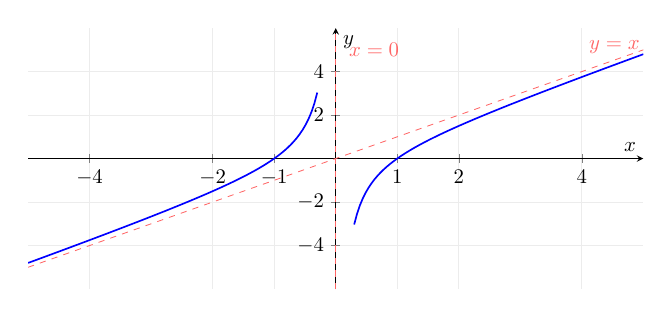
\begin{tikzpicture}[scale=0.75]
\begin{axis}[
    width=12cm, height=6cm,
    axis lines=middle,
    xlabel=$x$, ylabel=$y$,
    xmin=-5, xmax=5, ymin=-6, ymax=6,
    xtick={-4,-2,-1,1,2,4},
    ytick={-4,-2,2,4},
    grid=major, grid style={gray!15},
]
\addplot[thick,blue,domain=0.3:5,samples=100] {x-1/x};
\addplot[thick,blue,domain=-5:-0.3,samples=100] {x-1/x};
\draw[dashed,red!60] (axis cs:0,-6) -- (axis cs:0,6);
\node[red!60,right] at (axis cs:0.1,5) {$x=0$};
\draw[dashed,red!60] (axis cs:-5,-5) -- (axis cs:5,5);
\node[red!60,above right] at (axis cs:4,4.5) {$y=x$};
\end{axis}
\end{tikzpicture}
\end{center}
\end{frame}


\begin{frame}[t]
	13. 如图，\(\triangle OAB\) 是边长为 2 的正三角形，记 \(\triangle OAB\) 位于直线 \(x=t (t>0)\) 左侧的图形的面积为 \(f(t)\)。试求函数 \(y=f(t)\) 的解析式，并画出函数 \(y=f(t)\) 的图象。
	
	\vspace{2em}\medskip
	\begin{center}	
	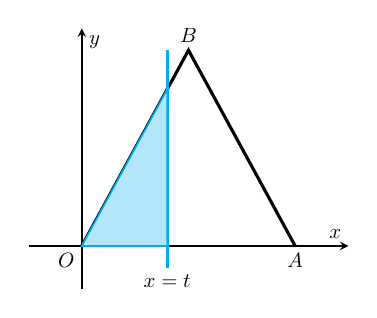
\begin{tikzpicture}[scale=0.75]
		\begin{axis}[
			width=7cm, height=6cm,
			axis lines=middle,
			xlabel=$x$, ylabel=$y$,
			xmin=-1, xmax=5, ymin=-1, ymax=5,
			xtick={0},
			ytick={0},
			axis line style={thick},
%			grid=major, grid style={gray!15},
			]
			\addplot[line width=1.5pt,black,name path = cur] coordinates{(0,0) (2,4.5)(4,0)};
			\addplot[line width=1.5pt,cyan,name path =line] coordinates{(1.6,-0.5) (1.6,4.5)};
			\path[name intersections={of=cur and line,by=point}];
			\draw[cyan,thick,fill=cyan!30] (0,0) -- (point) -- (point |- 0,0) --cycle;
			\node [below left] at (0,0) {$O$};
			\node [above] at (2,4.5) {$B$};
			\node [below] at (4,0) {$A$};
			\node [below] at (1.6,-0.5){$x=t$};
		\end{axis}
	\end{tikzpicture}
\end{center}
\end{frame}

\begin{frame}
	\begin{tcolorbox}[colback=orange!10,colframe=orange,title=\textbf{解}]
		\(\triangle OAB\) 是边长为 2 的正三角形，且 \(O\) 为原点，边 \(OA\) 在 \(x\) 轴上。
		
		由正三角形性质可知，点 \(A\) 的坐标为 \((2, 0)\)，点 \(B\) 的横坐标为 1，纵坐标为 \(2 \times \sin 60^\circ = \sqrt{3}\)，即 \(B(1, \sqrt{3})\)。
		
		直线 \(OB\) 的方程为：\(y = \sqrt{3}x \quad (0 \le x \le 1)\)
		
		直线 \(AB\) 的方程为：\(y = -\sqrt{3}(x-2) = -\sqrt{3}x + 2\sqrt{3} \quad (1 \le x \le 2)\)
		
		我们需要根据直线 \(x=t\) 的位置分段讨论面积 \(f(t)\)：
		
		\begin{enumerate}
			\item \textbf{当 \(0 < t \le 1\) 时：}
			
			直线 \(x=t\) 与边 \(OB\) 相交，交点的纵坐标为 \(\sqrt{3}t\)。
			
			此时左侧图形是一个直角三角形，其底为 \(t\)，高为 \(\sqrt{3}t\)。
			\[
			f(t) = \frac{1}{2} \cdot t \cdot \sqrt{3}t = \frac{\sqrt{3}}{2}t^2
			\]
			
		
		\end{enumerate}
		\end{tcolorbox}
		
		
\end{frame}

\begin{frame}
	\vspace{-1em}
	\begin{tcolorbox}[colback=orange!10,colframe=orange,title=\textbf{接上页}]			
		\begin{enumerate}
			\setcounter{enumi}{1}			
			\item \textbf{当 \(1 < t \le 2\) 时：}
			
			直线 \(x=t\) 左侧的图形由\textbf{一个三角形和一个直角梯形}组成（以 \(x=1\) 为界）：
			\begin{itemize}
				\item \textbf{左侧三角形面积}：底为 1，高为 \(\sqrt{3}\)，面积为 \(S_1 = \frac{1}{2} \times 1 \times \sqrt{3} = \frac{\sqrt{3}}{2}\)。
				\item \textbf{右侧梯形面积}：上底为 \(\sqrt{3}\)（点 \(B\) 的纵坐标），下底为直线 \(x=t\) 与 \(AB\) 交点纵坐标 \(-\sqrt{3}t + 2\sqrt{3}\)，高为 \(t-1\)。
				\[
				S_2 = \frac{1}{2} \left[ \sqrt{3} + (-\sqrt{3}t + 2\sqrt{3}) \right] \cdot (t-1) = \frac{1}{2} (3\sqrt{3} - \sqrt{3}t)(t-1)
				\]
			\end{itemize}
			总面积为：
			\begin{align*}
				f(t) &= S_1 + S_2 \\
				&= \frac{\sqrt{3}}{2} + \frac{\sqrt{3}}{2}(3-t)(t-1) \\
%				&= \frac{\sqrt{3}}{2} \left[ 1 + (3t - 3 - t^2 + t) \right] \\
%				&= \frac{\sqrt{3}}{2} (-t^2 + 4t - 2) \\
				&= -\frac{\sqrt{3}}{2}t^2 + 2\sqrt{3}t - \sqrt{3}
			\end{align*}
			
			
		\end{enumerate}
		
	
	\end{tcolorbox}
	
	
\end{frame}

\begin{frame}[t]
	\vspace{-1em}
	\begin{tcolorbox}[colback=orange!10,colframe=orange,sidebyside,title=\textbf{接上页}]		
		
			\begin{enumerate}
			\setcounter{enumi}{2}			
			
			
			\item \textbf{当 \(t > 2\) 时：}
			
			直线 \(x=t\) 在点 \(A\) 右侧，覆盖了整个三角形。
			\[
			f(t) = S_{\triangle OAB} = \frac{\sqrt{3}}{4} \times 2^2 = \sqrt{3}
			\]
		\end{enumerate}	
		综上所述，函数解析式为：
		\[
		f(t) = \begin{cases} 
			\frac{\sqrt{3}}{2}t^2, & 0 < t \le 1 \\ 
			-\frac{\sqrt{3}}{2}t^2 + \frac{3\sqrt{3}}{2}t, & 1 < t \le 2 \\ 
			\sqrt{3}, & t > 2 
		\end{cases}
		\]
	\tcblower
	函数$f(t)$的图象为：
	\begin{center}
		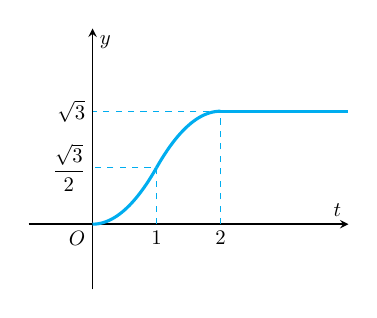
\begin{tikzpicture}[scale=0.75]
			\begin{axis}[
				width=7cm, height=6cm,
				axis lines=middle,
				xlabel=$t$, ylabel=$y$,
				xmin=-1, xmax=4, ymin=-1, ymax=3,
				xtick={0},
				ytick={0},
				axis line style={thick},
				%			grid=major, grid style={gray!15},
				]
				\addplot[line width=1.5pt,cyan,domain=0:1] {sqrt(3)/2*x^2};
				\addplot[line width=1.5pt,cyan,domain=1:2] {-sqrt(3)/2*x^2+2*sqrt(3)*x-sqrt(3)};
				\addplot[line width=1.5pt,cyan] coordinates {(2,{sqrt(3)}) (4,{sqrt(3)})};
				\addplot[dashed,cyan] coordinates{(1,0) (1,{sqrt(3)/2}) (0,{sqrt(3)/2})};
				\addplot[dashed,cyan] coordinates{(2,0) (2,{sqrt(3)}) (0,{sqrt(3)})};
				\node [below left] at (0,0) {$O$};
				\node[below] at (1,0) {1};
				\node[below] at  (2,0) {2};
				\node[left] at (0,{sqrt(3)}) {$\sqrt{3}$};
				\node[left] at (0,{sqrt(3)/2}) {$\dfrac{\sqrt{3}}{2}$};
				
			\end{axis}
		\end{tikzpicture}
	\end{center}
	\end{tcolorbox}
\end{frame}


\begin{frame}[t]
	14. 某商场经营一批进价为 30 元/件的商品，在市场试销中发现，此商品的销售单价 \(x\)（单位：元）与日销售量 \(y\)（单位：件）之间有如下表所示的关系。
	
	\begin{center}
		\begin{tabular}{|c|c|c|c|c|c|c|}
			\hline
			\(x\) & \(\cdots\) & 30 & 40 & 45 & 50 & \(\cdots\) \\
			\hline
			\(y\) & \(\cdots\) & 60 & 30 & 15 & 0 & \(\cdots\) \\
			\hline
		\end{tabular}
	\end{center}
	
	\begin{enumerate}
		\item[(1)] 根据表中提供的数据描出实数对 \((x, y)\) 的对应点，根据画出的点猜想 \(y\) 与 \(x\) 之间的函数关系，并写出一个函数解析式；
		\item[(2)] 设经营此商品的日销售利润为 \(P\)（单位：元），根据上述关系，写出 \(P\) 关于 \(x\) 的函数解析式，并求销售单价为多少元时，才能获得最大日销售利润。
	\end{enumerate}
\end{frame}

\begin{frame}
	\begin{tcolorbox}[colback=orange!10,colframe=orange,title=\textbf{解：}]		
		\textbf{(1)} 描点略。观察表格数据：
		
		\begin{itemize}
			\item \(x\) 从 30 增加到 40，增加 10，\(y\) 从 60 减少到 30，减少 30。
			\item \(x\) 从 40 增加到 45，增加 5，\(y\) 从 30 减少到 15，减少 15。
			\item \(x\) 从 45 增加到 50，增加 5，\(y\) 从 15 减少到 0，减少 15。
		\end{itemize}
		
		可以看出 \(y\) 随 \(x\) 的变化率是常数，即 \(\frac{\Delta y}{\Delta x} = \frac{30-60}{40-30} = -3\)。
		
		因此猜想 \(y\) 与 \(x\) 之间是一次函数关系。设 \(y = kx + b\)。
		
		代入点 \((50, 0)\) 和 \((40, 30)\)：
		\[
		\begin{cases} 
			50k + b = 0 \\ 
			40k + b = 30 
		\end{cases}
		\]
		解得 \(k = -3, b = 150\)。
		
		所以函数解析式为：\textbf{\(y = -3x + 150\)}。
		
		
		
	\end{tcolorbox}
\end{frame}

\begin{frame}
	\begin{tcolorbox}[colback=orange!10,colframe=orange,sidebyside,title=\textbf{解：}]		
		
		
		\textbf{(2)} 日销售利润 \(P = (\text{销售单价} - \text{进价}) \times \text{日销售量}\)。
		
		已知进价为 30 元/件，销售单价为 \(x\) 元，销售量为 \(y = -3x + 150\) 件。
		\begin{align*}
			P &= (x - 30)y \\
			&= (x - 30)(-3x + 150) \\
			&= -3x^2 + 150x + 90x - 4500 \\
			&= -3x^2 + 240x - 4500
		\end{align*}
		配方求最值：
		\tcblower
		
		\begin{align*}
			P &= -3(x^2 - 80x) - 4500 \\
%			&= -3(x^2 - 80x + 1600 - 1600) - 4500 \\
%			&= -3(x - 40)^2 + 4800 - 4500 \\
			&= -3(x - 40)^2 + 300
		\end{align*}
		
		因为 \(-3 < 0\)，所以当 \(x = 40\) 时，\(P\) 取得最大值，最大值为 300 元。
		
		\textbf{答：}
		\(P\) 关于 \(x\) 的函数解析式为 \(P = -3x^2 + 240x - 4500\)（且由 \(y \ge 0\) 得 \(30 \le x \le 50\)）。
		
		当销售单价为 \textbf{40 元} 时，才能获得最大日销售利润，最大利润为 \textbf{300 元}。
		
	\end{tcolorbox}
\end{frame}


\begin{frame}[c]
	\begin{center}
		{\Huge\calligra Thanks!}
	\end{center}
\end{frame}

\end{document}
